
\begin{figure*}[ht]
    \centering
    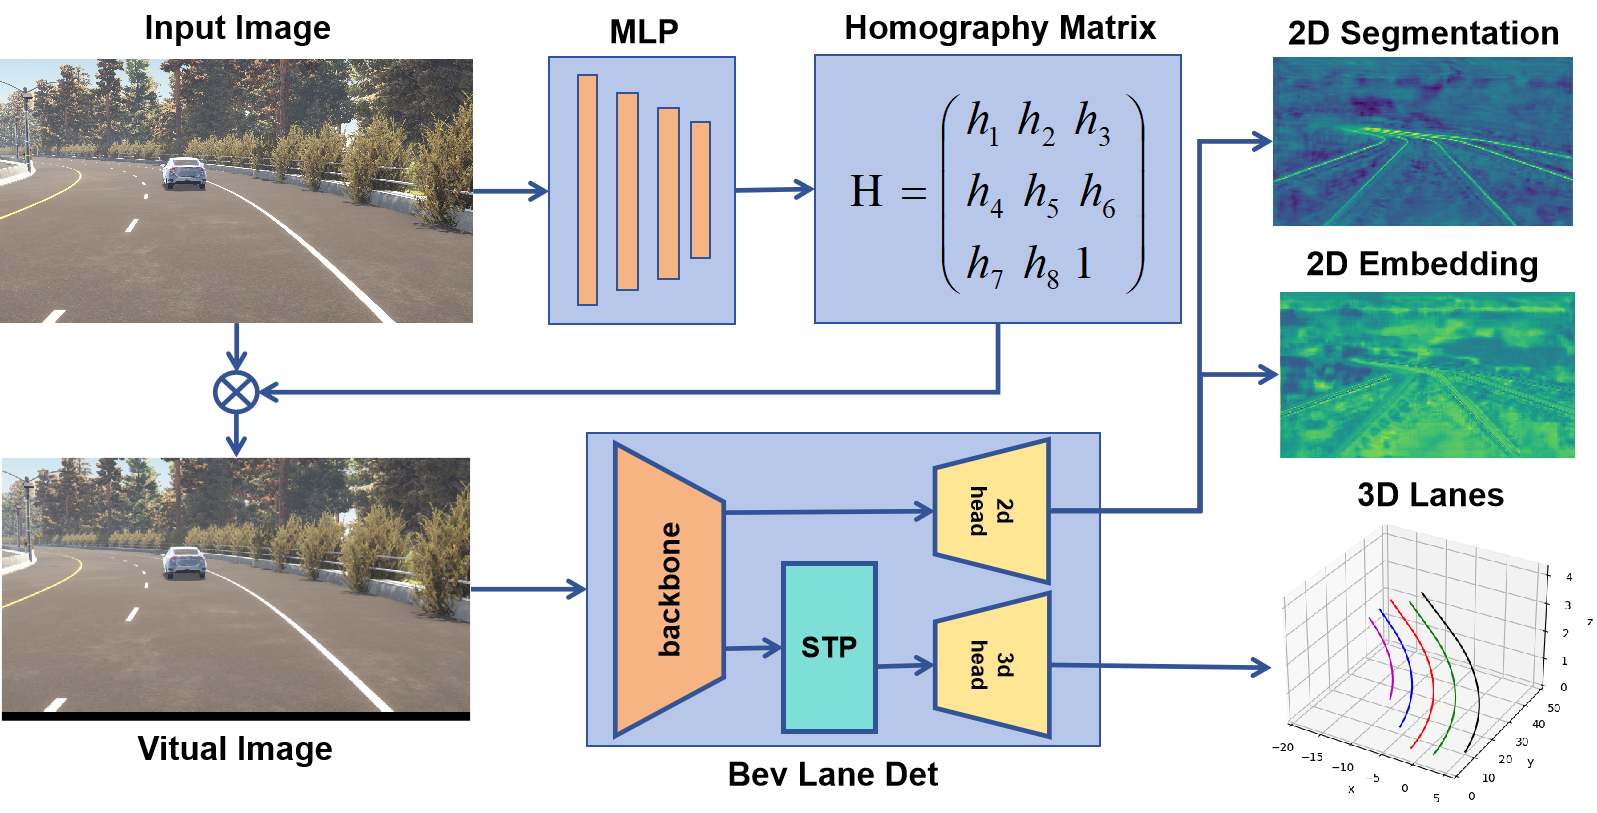
\includegraphics[height=0.45\textheight]{asset/structure} %width=1\linewidth
    \caption{Overview of the framework}
    \label{fig:overview}
\end{figure*}

\section{Methods}
\label{sec:methods}
%Fig.\ref{fig:overview} shows the overview of our entire lane detection framework.
An overview of our entire lane detection framework is illustrated in Fig.\ref{fig:overview}.
Our approach takes a single image captured by a front camera mounted on the vehicle as input information.
The image from the current camera is projected onto the view of the virtual camera using the homography
matrix generated by MLP network \cite{tang2022image},
which aims to transform the in/external parameters of the input image to a unified
in/external parameter of the virtual camera.
We use ResNet18 and ResNet34 \cite{he2016deep} as our backbone to extract front view image features.
Spatial Transformation Pyramid \cite{wang2023bev} transform the front view features into BEV features.
Then, lanes are predicted on the BEV view. We predict the confidence of each cell, the embedding used for clustering,
the offset from the center of the cell to the lane in the y-direction, and the height.
we added the front view lane detection header as an
auxiliary supervision to improve backbone's ability to extract front view features
and supervise the homography matrix estimation network's training.

\subsection{Homography}
new
why use homography?
If a fixed transformation matrix is employed, the projection becomes less accurate when sloping ground planes or camera vibrations are encountered.
To remedy this situation, we train a network to output certain crucial parameters in the perspective transformation.

101
011
001
A full projection model describes the mapping from world to pixel coordinates.
For this nonlinear projection, more unknown model parameters mean a higher risk of unstable output.
Fully constructing a 3 × 3 homographic matrix needs 8 dependent components.
However, treating each of them as an independent parameter is not a good idea since they are actually correlated.
Therefore, we set up a homographic model from the fundamental projection principle and try to reduce the number of outputs to the least degrees of freedom in H.
Depending on whether the camera is pre-calibrated, different outputs of the model are designed.

The zeros are placed to enforce the constraint that horizontal lines remain horizontal under the transformation.

old
A homography is a projective transformation between two planes or, alternatively, a mapping between two planar projections of an image.
In other words, homographies are simple image transformations that describe the relative motion between two images, when the camera (or the observed object) moves.
It is the simplest kind of transformation that describes the 2D relationship between two images.
Homography can be mathematically described by a 3D transformation in a homogeneous coordinates space and can be expressed as:

\[
S\left[ \begin{matrix}
   x'  \\
   y'  \\
   1
\end{matrix} \right]
=
H\left[ \begin{matrix}
   x  \\
   y  \\
   1
\end{matrix} \right]
=
\left[ \begin{matrix}
h_1 & h_2 & h_3  \\
h_4 & h_5 & h_6  \\
h_7 & h_8 & h_9  \\
\end{matrix} \right]
\left[ \begin{matrix}
x  \\
y  \\
1
\end{matrix} \right]
\]
where H denotes the homography matrix $H \in R^{3\times 3}$ between two two-dimensional planes,
which allows us to switch from one view of the same scene to another by multiplying
the homography matrix with the points [u,v] in one view to find their corresponding positions [u',v'] in the other view.
The homography matrix is usually parameterized by the elements of a 3×3 matrix,
but it has only 8 degrees of freedom, and a simple way to do this is to hardcode $h_9=1$.
We take the original image as input and use DNN to estimate eight parameters of the homography matrix.


\begin{figure}[!ht]
    \centering
    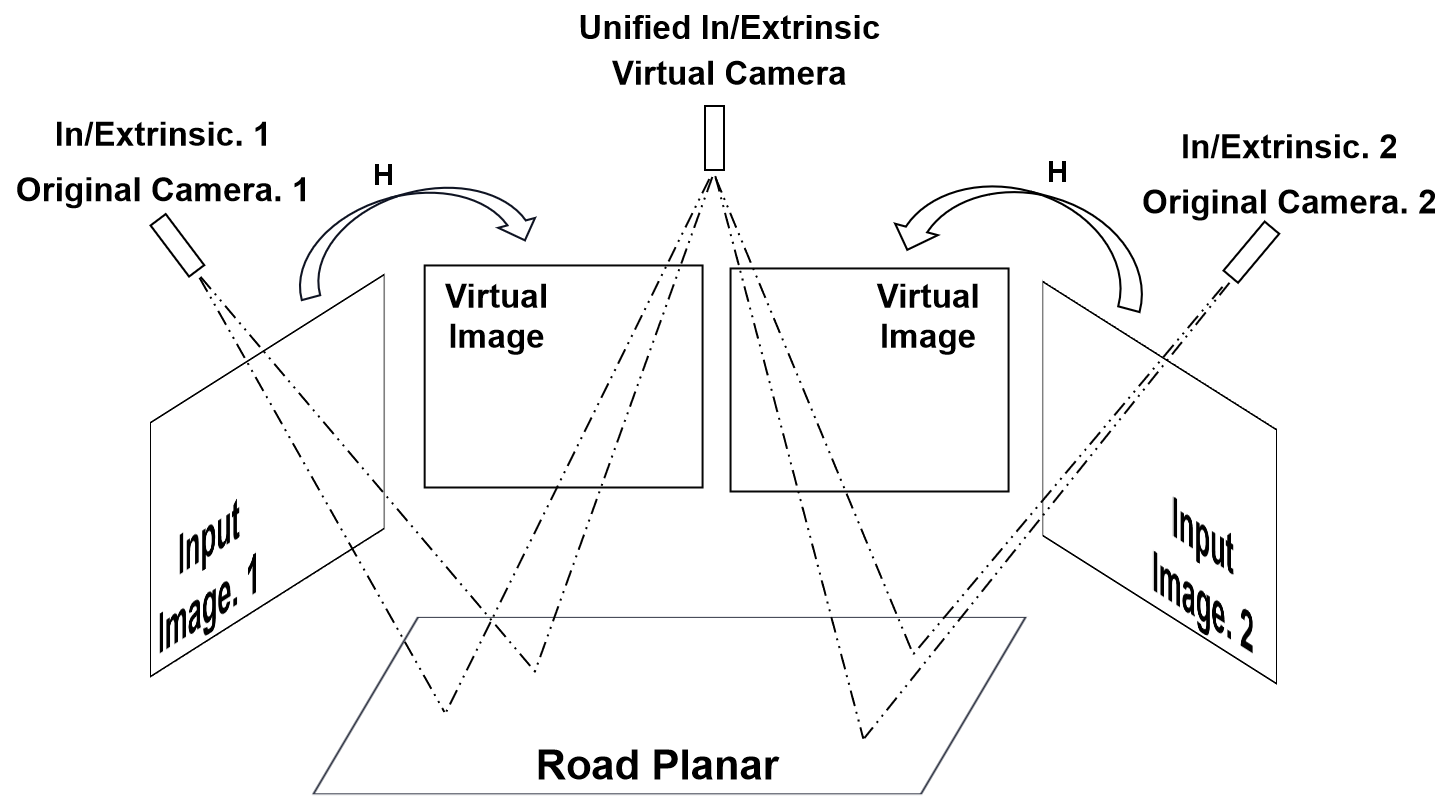
\includegraphics[width=\linewidth]{asset/virtual_camera}
    \caption{Virtual Camera}
    \label{fig:Virtual Camera}
\end{figure}

\begin{figure*}[!ht]
    \centering
    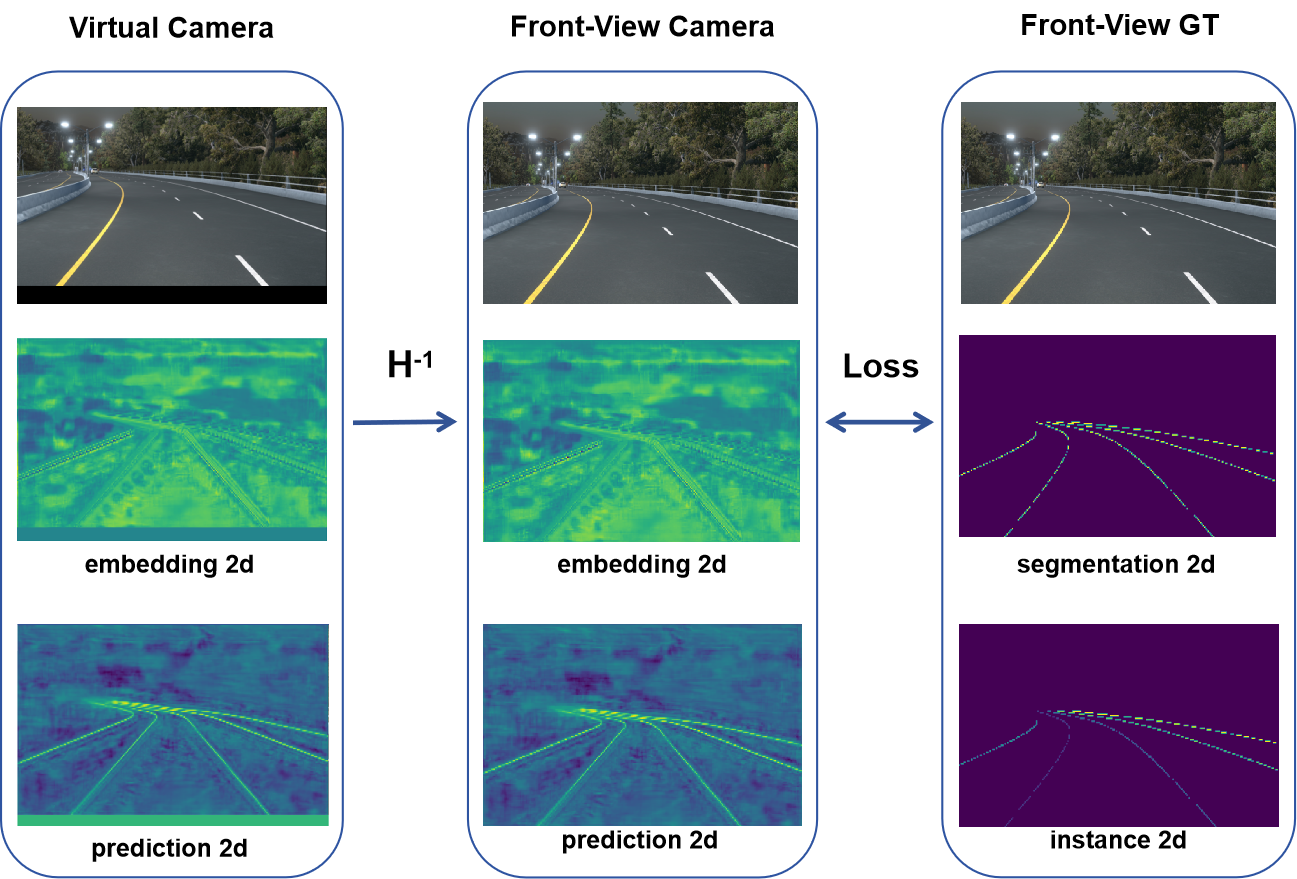
\includegraphics[height=0.45\textheight]{asset/loss2}
    \caption{Homography Loss}
    \label{fig:Homography Loss}
\end{figure*}

\subsection{Unified Camera Parameters}
\label{subsec:Unified Camera Parameters}
Different cameras mounted on the vehicle have different internal/external parameters,
which have a significant effect on the 3D lane results.
As shown in Fig.\ref{fig:Virtual Camera},
By creating a virtual camera with standard internal/external parameters,
we can unify the internal/external parameters of different cameras.
We project the image of the current camera into the view of the virtual camera through the homography matrix H based on the principle of perspective transformation.
As a result, the virtual camera unifies the internal/external parameters of different cameras.
%Wave-MLP  \cite{tang2022image} represents each token as a wave function with two parts,
%amplitude and phase, which can model different contents from different input images.
We use a MLP network to estimate the 8 parameters of the homography matrix from the input frames.
Then, we transform from one view of the same scene to another by multiplying the homography matrix with the points $[u,v]$ in one view
to find their corresponding locations $[u',v']$ in the other view.

\subsection{Homography Loss}
\label{subsec:Homography Loss}
as shown in Fig.\ref{fig:Homography Loss}. In order to improve the MLP network's ability to extract homography matrix parameters and backbone's ability to extract front view features,
a front view lane detection header was added as an auxiliary supervision.
Based on this front view lane detection head, we propose the homography loss function.
After the input image is converted to a virtual camera image by homography matrix $H$,
the front view features of the virtual camera image are obtained by backbone,
and the front view lane detection head gets the virtual camera segmentation and embedding results ${Seg}_{v}, {Emb}_{v}$,
which can be converted back to the input camera ${Seg}_{i}, {Emb}_{i}$ by the inverse matrix $H^{-1}$ of the homography matrix.
The front-view lane loss includes lane segmentation loss and lane embedding loss, referred to LaneNet \cite{neven2018towards}.The homography loss is defined as follows,
\[
L_{h}=\lambda_{seg}^h L_{seg}^h + \lambda_{emb}^h L_{emb}^h
\]
where $L_{seg}^h$ denotes lane segmentation loss, and$L_{emb}^h$ denotes lane embedding loss in the front-view.
